\documentclass[final,t]{beamer}
\mode<presentation>{\usetheme{default}}
\usepackage{type1cm}
\usepackage{fix-cm}
\usepackage{amsmath,amssymb}
\usepackage{etoolbox}
\usepackage{graphicx}
\usepackage{tikz}
\usetikzlibrary{arrows.meta, positioning, shapes.geometric, fit, calc}
\usepackage[orientation=portrait,size=a1,scale=1.2]{beamerposter}

% Color definitions
\definecolor{cDarkBlue}{rgb}{0, 0.2, 0.5}
\definecolor{headerblue}{rgb}{0.1, 0.2, 0.4}
\definecolor{rowsep}{rgb}{0.8, 0.8, 0.8}
\definecolor{lightblue}{rgb}{0.85, 0.9, 0.95}

% Poster metadata
\newcommand{\postertitle}{Making Safe Reinforcement Learning Faster}
\newcommand{\posterauthors}{Julius Landes, Christoph Mayer, Elias M\"uller, Laurin van den Bergh}

% Beamer settings
\setbeamercolor{block title}{fg=white,bg=cDarkBlue}
\setbeamercolor{block body}{fg=black,bg=white}
\setbeamercolor{headline}{fg=white,bg=headerblue}
\setbeamertemplate{navigation symbols}{}
\setbeamertemplate{footline}{}

\begin{document}
\begin{frame}[t]

%% ============================================
%% HEADER
%% ============================================
\vspace{-1cm}
\begin{beamercolorbox}[wd=\textwidth,ht=7cm,center]{headline}
\vspace{1cm}
{\Huge\textbf{\postertitle}}\\[0.8cm]
{\Large \posterauthors}
\end{beamercolorbox}

\vspace{0.5cm}

%% ============================================
%% ROW 1: MOTIVATION
%% ============================================
\begin{columns}[T]

\begin{column}{0.32\textwidth}
\begin{block}{Situation}
\textbf{Configurable Environments}\\[0.3cm]
Most Reinforcement Learning research focuses on \textbf{static MDPs}, where the environment dynamics are fixed.\\[0.3cm]
However, many real-world environments are \textbf{configurable}---certain parameters can be tuned to improve agent performance.\\[0.3cm]
\textbf{Configurable MDPs (Conf-MDPs)} extend standard MDPs by allowing the transition model $P$ to be selected from a space $\mathcal{P}$:
\[
\mathcal{CM} = (\mathcal{S}, \mathcal{A}, R, \gamma, \mu, \mathcal{P}, \Pi)
\]
\end{block}
\end{column}

\begin{column}{0.32\textwidth}
\begin{block}{Example}
\textbf{Car Configuration}\\[0.3cm]
Consider a car with \textbf{sport} and \textbf{comfort} driving modes:
\begin{itemize}
    \item \textbf{Sport mode:} Aggressive acceleration, less stability
    \item \textbf{Comfort mode:} Smooth driving, better control
\end{itemize}
\vspace{0.3cm}
On a \textbf{slippery road}, the optimal configuration depends on the driving policy---and vice versa.\\[0.3cm]
The goal: \textbf{jointly optimize} the policy $\pi$ and environment configuration $P$ to maximize expected return $J_\mu^{P,\pi}$.
\end{block}
\end{column}

\begin{column}{0.32\textwidth}
\begin{block}{Problem \& Solution}
\textbf{The Challenge}\\[0.3cm]
\textbf{SPMI} (Safe Policy-Model Iteration) provides \textbf{monotonic improvement guarantees} but is computationally expensive.\\[0.3cm]
\textbf{Our Solution: Federated Learning}\\[0.3cm]
We propose \textbf{F-SPMI} (Federated SPMI):
\begin{itemize}
    \item Multiple agents explore in parallel
    \item Agents share learned value functions
    \item Central server aggregates knowledge
    \item \textbf{Safety guarantees preserved}
\end{itemize}
\vspace{0.3cm}
\textit{Faster learning through collaboration while maintaining safety!}
\end{block}
\end{column}

\end{columns}

\vspace{0.3cm}
\textcolor{rowsep}{\rule{\textwidth}{2pt}}
\vspace{0.3cm}

%% ============================================
%% ROW 2: THEORY
%% ============================================
\begin{columns}[T]

\begin{column}{0.48\textwidth}
\begin{block}{F-SPMI Architecture}
\vspace{0.3cm}
\begin{center}
\begin{tikzpicture}[scale=1.0, transform shape,
    agent/.style={rectangle, draw=cDarkBlue, fill=lightblue, thick, minimum width=2.8cm, minimum height=1.5cm, align=center},
    server/.style={rectangle, draw=cDarkBlue, fill=cDarkBlue!20, thick, minimum width=4cm, minimum height=2.5cm, align=center},
    output/.style={rectangle, draw=cDarkBlue, fill=cDarkBlue!10, thick, minimum width=3cm, minimum height=1.5cm, align=center},
    arrow/.style={-{Stealth[length=3mm]}, thick, cDarkBlue},
    labelstyle/.style={font=\normalsize, fill=white, inner sep=2pt}
]
% Agents (left side, well spaced)
\node[agent] (a1) at (0, 4) {Agent 1};
\node[agent] (a2) at (0, 2) {Agent 2};
\node[agent] (a3) at (0, 0) {Agent $N$};
\node at (0, 1) {\Large$\vdots$};

% Server (center - moved further right)
\node[server] (server) at (10, 2) {\textbf{Central Server}\\[0.2cm]Aggregation\\$\hat{Q}, \hat{\delta}, \hat{U}$};

% Output (right side - moved further right)
\node[output] (out) at (17, 2) {Updated\\$(P_{k+1}, \pi_{k+1})$};

% Arrows from agents to server
\draw[arrow] (a1.east) -- (server.165);
\draw[arrow] (a2.east) -- (server.west);
\draw[arrow] (a3.east) -- (server.195);

% Labels on arrows (larger font, centered between agents and server)
\node[labelstyle] at (5, 3.6) {$\hat{Q}_1, \hat{\delta}_1, \hat{U}_1$};
\node[labelstyle] at (5, 2) {$\hat{Q}_2, \hat{\delta}_2, \hat{U}_2$};
\node[labelstyle] at (5, 0.4) {$\hat{Q}_N, \hat{\delta}_N, \hat{U}_N$};

% Arrow from server to output
\draw[arrow] (server.east) -- node[above, labelstyle, yshift=50pt] {\textbf{Safe Update}} (out.west);

% Feedback loop - arrows come into agents from the left
\coordinate (feedbackBottom) at (8.5, -1.3);
\coordinate (feedbackLeft) at (-3, -1.3);
\draw[thick, dashed, cDarkBlue] (out.south) -- ++(0, -1.3) -- (feedbackLeft) -- (-3, 2);
\draw[arrow, dashed] (-3, 4) -- (a1.west);
\draw[arrow, dashed] (-3, 2) -- (a2.west);
\draw[arrow, dashed] (-3, 0) -- (a3.west);
\node[labelstyle] at (6, -1.9) {\textbf{Broadcast} $(P_{k+1}, \pi_{k+1})$ to all agents};

\end{tikzpicture}
\end{center}
\vspace{0.3cm}
\textbf{Local Statistics} (per agent $j$):
\begin{itemize}
    \item $\hat{Q}_j^{P_k, \pi_k}$: Q-function via Monte Carlo
    \item $\hat{\delta}_{\mu,j}^{P_k, \pi_k}$: $\gamma$-discounted state-action distribution
    \item $\hat{U}_j^{P_k, \pi_k}$: U-function estimate
\end{itemize}
\end{block}

\begin{block}{GP-Enhanced Model Selection}
Replace greedy model choice with \textbf{Gaussian Process UCB}:
\begin{equation*}
P_{k+1} = \arg\max_{P \in \mathcal{P}} \left[ \mu(P) + \beta_k \sigma(P) \right]
\end{equation*}
Balances \textit{exploitation} (high predicted advantage $\mu$) with \textit{exploration} (high uncertainty $\sigma$) for principled model space search.
\end{block}
\end{column}

\begin{column}{0.48\textwidth}
\begin{block}{Safe Update Mechanism}
\vspace{0.3cm}
\textbf{Weighted Federated Averaging}\\[0.2cm]
The server aggregates local estimates:
\begin{equation*}
\hat{Q}^{P_k, \pi_k}(s,a) = \frac{\sum_{j=1}^N M_j(s,a) \hat{Q}_j^{P_k, \pi_k}(s,a)}{\sum_{j=1}^N M_j(s,a)}
\end{equation*}
where $M_j(s,a)$ is the visit count by agent $j$.\\[0.4cm]

\textbf{Decoupled Bound} (Theorem 3.3, Metelli et al.)\\[0.2cm]
Performance improvement is lower bounded:
\begin{equation*}
J_\mu^{P', \pi'} - J_\mu^{P, \pi} \geq \underbrace{\frac{A_{P,\pi,\mu}^{P',\pi} + A_{P,\pi,\mu}^{P,\pi'}}{1-\gamma}}_{\text{advantage}} - \underbrace{\frac{\gamma \Delta Q^{P,\pi} D}{2(1-\gamma)^2}}_{\text{penalization}}
\end{equation*}

\textbf{Safe Step Sizes}\\[0.2cm]
Optimal update coefficients:
\begin{equation*}
\alpha^*, \beta^* = \arg\max_{\alpha,\beta} \hat{B}(\alpha, \beta)
\end{equation*}
ensuring \textbf{monotonic performance improvement}.
\end{block}
\end{column}

\end{columns}

\vspace{0.3cm}
\textcolor{rowsep}{\rule{\textwidth}{2pt}}
\vspace{0.3cm}

%% ============================================
%% ROW 3: EXPERIMENTAL RESULTS
%% ============================================
\begin{columns}[T]

\begin{column}{0.48\textwidth}
\begin{block}{Convergence Results}
\begin{center}
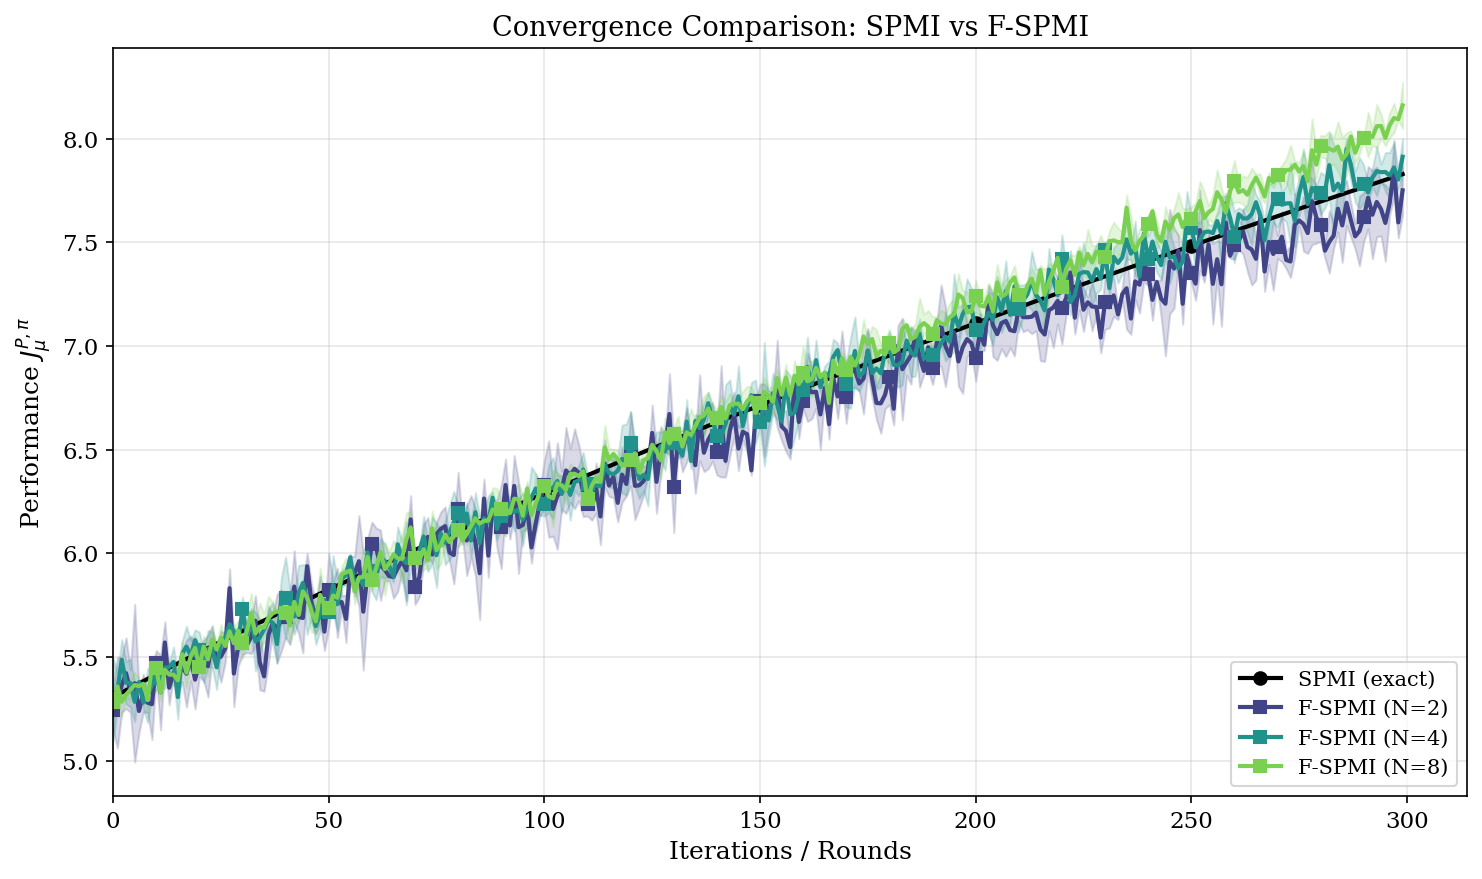
\includegraphics[width=0.95\linewidth]{experiments/results_300_8/convergence_comparison.png}
\end{center}
\vspace{0.2cm}
F-SPMI (colored lines) successfully tracks the optimal trajectory of \textbf{Exact SPMI} (black line), converging to return $\approx 7.1$.
\end{block}
\end{column}

\begin{column}{0.48\textwidth}
\begin{block}{Performance Analysis}
\begin{center}
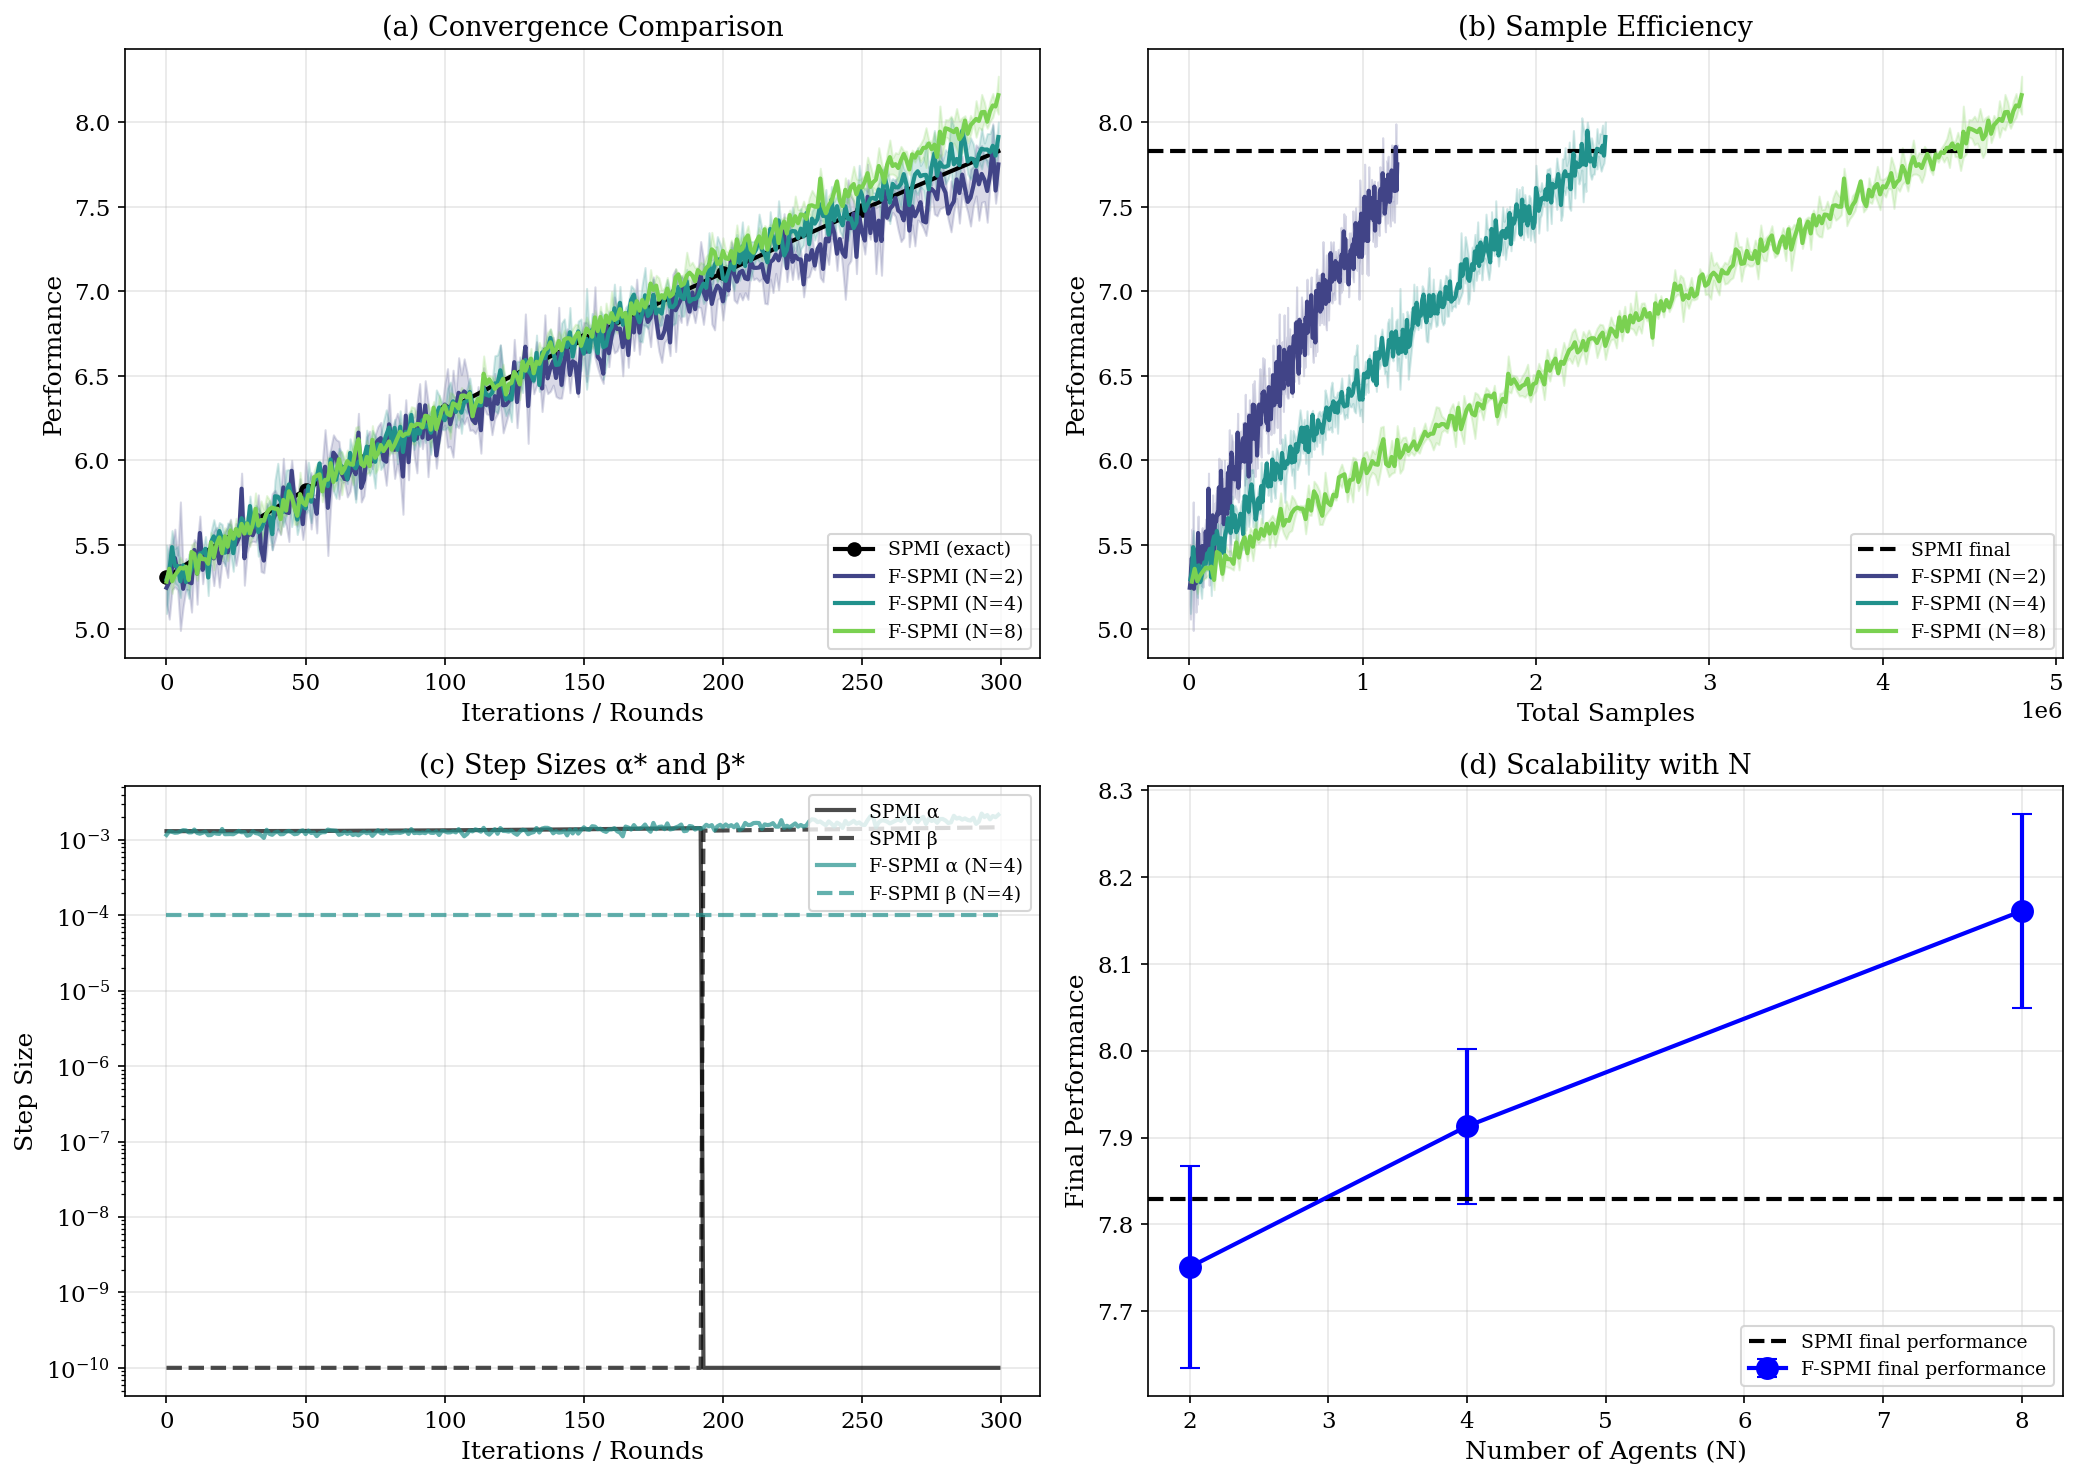
\includegraphics[width=0.95\linewidth]{experiments/results_300_8/summary_figure.png}
\end{center}
\vspace{0.2cm}
\textbf{Key Findings:} (a) Convergence, (b) Sample efficiency, (c) Step sizes $\alpha, \beta$, (d) Scalability with $N$ agents.
\end{block}
\end{column}

\end{columns}

\vspace{0.3cm}
\textcolor{rowsep}{\rule{\textwidth}{2pt}}
\vspace{0.3cm}

%% ============================================
%% ROW 4: CONCLUSION
%% ============================================
\begin{columns}[T]

\begin{column}{0.32\textwidth}
\begin{block}{Summary}
\textbf{Key Contributions:}
\begin{itemize}
    \item F-SPMI enables \textbf{parallel safe RL} in configurable environments
    \item Maintains \textbf{monotonic improvement} guarantees from SPMI
    \item \textbf{Robust to noise}: Sample-based estimates converge to optimal
    \item Optional \textbf{GP-UCB} model selection for principled exploration
\end{itemize}
\end{block}
\end{column}

\begin{column}{0.32\textwidth}
\begin{block}{Limitations}
\textbf{Current Constraints:}
\begin{itemize}
    \item Requires \textbf{known model space} $\mathcal{P}$
    \item Communication overhead between agents and server
    \item Discrete state-action spaces in current implementation
    \item Synchronous updates across all agents
\end{itemize}
\end{block}
\end{column}

\begin{column}{0.32\textwidth}
\begin{block}{Outlook}
\textbf{Future Directions:}
\begin{itemize}
    \item \textbf{Sample-based} extension without known model space
    \item \textbf{Continuous} state-action spaces via policy gradient methods
    \item Asynchronous federated updates
    \item Application to real-world robotics and autonomous systems
\end{itemize}
\end{block}
\end{column}

\end{columns}

\vspace{0.5cm}
\begin{center}
\small\textit{Reference: Metelli et al., ``Configurable Markov Decision Processes'', ICML 2018}
\end{center}

\end{frame}
\end{document}
